\documentclass{anstrans}

\title{Safety Analysis of the Molten Salt Fast Reactor Fuel Composition using Moltres}
\author{Sun Myung Park$^{a,b}$, Andrei Rykhlevskii$^a$, and Kathryn D. Huff$^a$}
\institute{$^a$Dept. of Nuclear, Plasma and Radiological Engineering, University of Illinois at Urbana-Champaign \\
$^b$smpark3@illinois.edu}

\usepackage{graphicx} % allows inclusion of graphics
\usepackage{booktabs} % nice rules (thick lines) for tables
\usepackage{microtype} % improves typography for PDF
\usepackage{float}
\usepackage{longtable}
\usepackage{xspace}
\usepackage{multirow} 
\usepackage{array}
\setlength{\arrayrulewidth}{.4mm}
\renewcommand{\arraystretch}{1.2}
\usepackage[labelfont=bf]{caption}
%\captionsetup[table]{name=Table}
\renewcommand{\thetable}{\arabic{table}}
\usepackage{caption}
\usepackage{subcaption}
\usepackage{enumitem}
\usepackage{placeins}
\usepackage{siunitx}
\newcolumntype{c}{>{\hsize=.56\hsize}X}
\newcolumntype{b}{>{\hsize=.7\hsize}X}
%\newcolumntype{s}{>{\hsize=.74\hsize}X}
\newcolumntype{f}{>{\hsize=.1\hsize}X}
\newcolumntype{a}{>{\hsize=.45\hsize}X}
\usepackage{titlesec}
\titleformat*{\subsection}{\normalfont}
\usepackage[super]{cite}
\usepackage{multirow}
\usepackage{hhline}


\usepackage[acronym,toc]{glossaries}
%\newacronym{<++>}{<++>}{<++>}
\newacronym[longplural={metric tons of heavy metal}]{MTHM}{MTHM}{metric ton of heavy metal}
\newacronym{ABM}{ABM}{agent-based modeling}
\newacronym{ACDIS}{ACDIS}{Program in Arms Control \& Domestic and International Security}
\newacronym{AHTR}{AHTR}{Advanced High Temperature Reactor}
\newacronym{ANDRA}{ANDRA}{Agence Nationale pour la gestion des D\'echets RAdioactifs, the French National Agency for Radioactive Waste Management}
\newacronym{ANL}{ANL}{Argonne National Laboratory}
\newacronym{API}{API}{application programming interface}
\newacronym{ARE}{ARE}{Aircraft Reactor Experiment}
\newacronym{ARFC}{ARFC}{Advanced Reactors and Fuel Cycles}
\newacronym{ASME}{ASME}{American Society of Mechanical Engineers}
\newacronym{ATWS}{ATWS}{Anticipated Transient Without Scram}
\newacronym{BDBE}{BDBE}{Beyond Design Basis Event}
\newacronym{BIDS}{BIDS}{Berkeley Institute for Data Science}
\newacronym{BOL}{BOL}{beginning of life}
\newacronym{CAFCA}{CAFCA}{ Code for Advanced Fuel Cycles Assessment }
\newacronym{CDTN}{CDTN}{Centro de Desenvolvimento da Tecnologia Nuclear}
\newacronym{CEA}{CEA}{Commissariat \`a l'\'Energie Atomique et aux \'Energies Alternatives}
\newacronym{CI}{CI}{continuous integration}
\newacronym{CNEN}{CNEN}{Comiss\~{a}o Nacional de Energia Nuclear}
\newacronym{CNERG}{CNERG}{Computational Nuclear Engineering Research Group}
\newacronym{COSI}{COSI}{Commelini-Sicard}
\newacronym{COTS}{COTS}{commercial, off-the-shelf}
\newacronym{CSNF}{CSNF}{commercial spent nuclear fuel}
\newacronym{CTAH}{CTAHs}{Coiled Tube Air Heaters}
\newacronym{CUBIT}{CUBIT}{CUBIT Geometry and Mesh Generation Toolkit}
\newacronym{CURIE}{CURIE}{Centralized Used Fuel Resource for Information Exchange}
\newacronym{DAG}{DAG}{directed acyclic graph}
\newacronym{DANESS}{DANESS}{Dynamic Analysis of Nuclear Energy System Strategies}
\newacronym{DBE}{DBE}{Design Basis Event}
\newacronym{DESAE}{DESAE}{Dynamic Analysis of Nuclear Energy Systems Strategies}
\newacronym{DHS}{DHS}{Department of Homeland Security}
\newacronym{DOE}{DOE}{Department of Energy}
\newacronym{DRACS}{DRACS}{Direct Reactor Auxiliary Cooling System}
\newacronym{DRE}{DRE}{dynamic resource exchange}
\newacronym{DSNF}{DSNF}{DOE spent nuclear fuel}
\newacronym{DYMOND}{DYMOND}{Dynamic Model of Nuclear Development }
\newacronym{EBS}{EBS}{Engineered Barrier System}
\newacronym{EDZ}{EDZ}{Excavation Disturbed Zone}
\newacronym{EIA}{EIA}{U.S. Energy Information Administration}
\newacronym{EOL}{EOL}{end of life}
\newacronym{EPA}{EPA}{Environmental Protection Agency}
\newacronym{EP}{EP}{Engineering Physics}
\newacronym{FCO}{FCO}{Fuel Cycle Options}
\newacronym{FCT}{FCT}{Fuel Cycle Technology}
\newacronym{FEHM}{FEHM}{Finite Element Heat and Mass Transfer}
\newacronym{FEPs}{FEPs}{Features, Events, and Processes}
\newacronym{FHR}{FHR}{Fluoride-Salt-Cooled High-Temperature Reactor}
\newacronym{FLiBe}{FLiBe}{Fluoride-Lithium-Beryllium}
\newacronym{GDSE}{GDSE}{Generic Disposal System Environment}
\newacronym{GDSM}{GDSM}{Generic Disposal System Model}
\newacronym{GENIUSv1}{GENIUSv1}{Global Evaluation of Nuclear Infrastructure Utilization Scenarios, Version 1}
\newacronym{GENIUSv2}{GENIUSv2}{Global Evaluation of Nuclear Infrastructure Utilization Scenarios, Version 2}
\newacronym{GENIUS}{GENIUS}{Global Evaluation of Nuclear Infrastructure Utilization Scenarios}
\newacronym{GPAM}{GPAM}{Generic Performance Assessment Model}
\newacronym{GRSAC}{GRSAC}{Graphite Reactor Severe Accident Code}
\newacronym{GUI}{GUI}{graphical user interface}
\newacronym{HLW}{HLW}{high level waste}
\newacronym{HPC}{HPC}{high-performance computing}
\newacronym{HTC}{HTC}{high-throughput computing}
\newacronym{HTGR}{HTGR}{High Temperature Gas-Cooled Reactor}
\newacronym{IAEA}{IAEA}{International Atomic Energy Agency}
\newacronym{IEMA}{IEMA}{Illinois Emergency Mangament Agency}
\newacronym{INL}{INL}{Idaho National Laboratory}
\newacronym{IPRR1}{IRP-R1}{Instituto de Pesquisas Radioativas Reator 1}
\newacronym{IRP}{IRP}{Integrated Research Project}
\newacronym{ISFSI}{ISFSI}{Independent Spent Fuel Storage Installation}
\newacronym{ISRG}{ISRG}{Independent Student Research Group}
\newacronym{JFNK}{JFNK}{Jacobian-Free Newton Krylov}
\newacronym{LANL}{LANL}{Los Alamos National Laboratory}
\newacronym{LBNL}{LBNL}{Lawrence Berkeley National Laboratory}
\newacronym{LCOE}{LCOE}{levelized cost of electricity}
\newacronym{LDRD}{LDRD}{laboratory directed research and development}
\newacronym{LFR}{LFR}{Lead-Cooled Fast Reactor}
\newacronym{LLNL}{LLNL}{Lawrence Livermore National Laboratory}
\newacronym{LMFBR}{LMFBR}{Liquid Metal Fast Breeder Reactor}
\newacronym{LOFC}{LOFC}{Loss of Forced Cooling}
\newacronym{LOHS}{LOHS}{Loss of Heat Sink}
\newacronym{LOLA}{LOLA}{Loss of Large Area}
\newacronym{LP}{LP}{linear program}
\newacronym{LWR}{LWR}{Light Water Reactor}
\newacronym{MA}{MA}{minor actinide}
\newacronym{MCNP}{MCNP}{Monte Carlo N-Particle code}
\newacronym{MILP}{MILP}{mixed-integer linear program}
\newacronym{MIT}{MIT}{the Massachusetts Institute of Technology}
\newacronym{MOAB}{MOAB}{Mesh-Oriented datABase}
\newacronym{MOOSE}{MOOSE}{Multiphysics Object-Oriented Simulation Environment}
\newacronym{MOX}{MOX}{mixed oxide}
\newacronym{MSBR}{MSBR}{Molten Salt Breeder Reactor}
\newacronym{MSFR}{MSFR}{Molten Salt Fast Reactor}
\newacronym{MSRE}{MSRE}{Molten Salt Reactor Experiment}
\newacronym{MSR}{MSR}{Molten Salt Reactor}
\newacronym{NAGRA}{NAGRA}{National Cooperative for the Disposal of Radioactive Waste}
\newacronym{NEAMS}{NEAMS}{Nuclear Engineering Advanced Modeling and Simulation}
\newacronym{NEUP}{NEUP}{Nuclear Energy University Programs}
\newacronym{NFCSim}{NFCSim}{Nuclear Fuel Cycle Simulator}
\newacronym{NGNP}{NGNP}{Next Generation Nuclear Plant}
\newacronym{NMWPC}{NMWPC}{Nuclear MW Per Capita}
\newacronym{NNSA}{NNSA}{National Nuclear Security Administration}
\newacronym{NPRE}{NPRE}{Department of Nuclear, Plasma, and Radiological Engineering}
\newacronym{NQA1}{NQA-1}{Nuclear Quality Assurance - 1}
\newacronym{NRC}{NRC}{Nuclear Regulatory Commission}
\newacronym{NSF}{NSF}{National Science Foundation}
\newacronym{NSSC}{NSSC}{Nuclear Science and Security Consortium}
\newacronym{NUWASTE}{NUWASTE}{Nuclear Waste Assessment System for Technical Evaluation}
\newacronym{NWF}{NWF}{Nuclear Waste Fund}
\newacronym{NWTRB}{NWTRB}{Nuclear Waste Technical Review Board}
\newacronym{OCRWM}{OCRWM}{Office of Civilian Radioactive Waste Management}
\newacronym{ORION}{ORION}{ORION}
\newacronym{ORNL}{ORNL}{Oak Ridge National Laboratory}
\newacronym{PARCS}{PARCS}{Purdue Advanced Reactor Core Simulator}
\newacronym{PBAHTR}{PB-AHTR}{Pebble Bed Advanced High Temperature Reactor}
\newacronym{PBFHR}{PB-FHR}{Pebble-Bed Fluoride-Salt-Cooled High-Temperature Reactor}
\newacronym{PEI}{PEI}{Peak Environmental Impact}
\newacronym{PH}{PRONGHORN}{PRONGHORN}
\newacronym{PRKE}{PRKE}{Point Reactor Kinetics Equations}
\newacronym{PSPG}{PSPG}{Pressure-Stabilizing/Petrov-Galerkin}
\newacronym{PWAR}{PWAR}{Pratt and Whitney Aircraft Reactor}
\newacronym{PWR}{PWR}{Pressurized Water Reactor}
\newacronym{PyNE}{PyNE}{Python toolkit for Nuclear Engineering}
\newacronym{PyRK}{PyRK}{Python for Reactor Kinetics}
\newacronym{QA}{QA}{quality assurance}
\newacronym{RDD}{RD\&D}{Research Development and Demonstration}
\newacronym{RD}{R\&D}{Research and Development}
\newacronym{RELAP}{RELAP}{Reactor Excursion and Leak Analysis Program}
\newacronym{RIA}{RIA}{Reactivity Insertion Accident}
\newacronym{RIF}{RIF}{Region-Institution-Facility}
\newacronym{SFR}{SFR}{Sodium-Cooled Fast Reactor}
\newacronym{SINDAG}{SINDA{\textbackslash}G}{Systems Improved Numerical Differencing Analyzer $\backslash$ Gaski}
\newacronym{SKB}{SKB}{Svensk K\"{a}rnbr\"{a}nslehantering AB}
\newacronym{SNF}{SNF}{spent nuclear fuel}
\newacronym{SNL}{SNL}{Sandia National Laboratory}
\newacronym{STC}{STC}{specific temperature change}
\newacronym{SUPG}{SUPG}{Streamline-Upwind/Petrov-Galerkin}
\newacronym{SWF}{SWF}{Separations and Waste Forms}
\newacronym{SWU}{SWU}{Separative Work Unit}
\newacronym{TRIGA}{TRIGA}{Training Research Isotope General Atomic}
\newacronym{TRISO}{TRISO}{Tristructural Isotropic}
\newacronym{TSM}{TSM}{Total System Model}
\newacronym{TSPA}{TSPA}{Total System Performance Assessment for the Yucca Mountain License Application}
\newacronym{ThOX}{ThOX}{thorium oxide}
\newacronym{UFD}{UFD}{Used Fuel Disposition}
\newacronym{ULOHS}{ULOHS}{Unprotected Loss of Heat Sink}
\newacronym{UML}{UML}{Unified Modeling Language}
\newacronym{UOX}{UOX}{uranium oxide}
\newacronym{UQ}{UQ}{uncertainty quantification}
\newacronym{US}{US}{United States}
\newacronym{UW}{UW}{University of Wisconsin}
\newacronym{VISION}{VISION}{the Verifiable Fuel Cycle Simulation Model}
\newacronym{VV}{V\&V}{verification and validation}
\newacronym{WIPP}{WIPP}{Waste Isolation Pilot Plant}
\newacronym{YMR}{YMR}{Yucca Mountain Repository Site}

\makeglossaries

\begin{document}

\begin{abstract}
%
    Abstract
\end{abstract}

\section{Introduction}

	\glspl{MSR} are a class of nuclear reactors that
	contain nuclear fuel dissolved and circulating in a molten salt coolant
	loop.
	They potentially possess the ability to run for extended 
    periods with minimal shutdown time due to online fuel reprocessing, which
    is a clear advantage over solid-fuelled reactors that require significant
    downtime for refuelling.
    Their proposed equilibrium fuel compositions differ substantially from
    start-up compositions due to burnup of initial fissile material and 
    breeding of new fissile material, but also fissile material feeds and 
    removal of fission products. Also, while \gls{BOL} fuel composition is
    largely dependent on the initial core loading, the long-term equilibrium
    fuel composition is determined by the type of feed.
    Since the changing fuel composition 
    impacts safety parameters (e.g. reactivity feedback coefficients), a 
    licensing case for this class of reactors  must fully characterize 
    those impacts.

	While numerous computational tools exist for conventional nuclear reactors, 
    \glspl{MSR} present unique computational challenges that many fail to 
    address effectively. \glspl{MSR} differ
    profoundly from conventional 
    solid-fuelled reactors, particularly in their neutronics and 
    thermal-hydraulics behaviors.  New \gls{MSR} simulation tools must 
    capture strong coupling between neutronics and thermal-hydraulics 
    exhibited by \gls{DNP} movement as well as strong 
    Doppler and density feedback in the fuel salt.  This paper investigates 
    the impact of changing fuel composition on safety parameters in the 
    \gls{MSFR} concept using a new simulation tool for \glspl{MSR}, Moltres 
    \cite{lindsay_introduction_2018}.
    
    Moltres is an open source coupled neutronics/thermal hydraulics simulation 
    application for simulating \glspl{MSR}. Built on the \gls{MOOSE} finite 
    element framework \cite{gaston_moose:_2009}, Moltres solves the coupled 
    time-dependent multi-group neutron diffusion, temperature, and 
    \gls{DNP} governing equations.  The temperature and \gls{DNP} equations
    fully 
    account for fuel advection as the fuel salt flows upwards through the 
    core.
    
    The \gls{MSFR} model studied in this paper is a reference design for a 
    fast-spectrum \gls{MSR} developed under H2020
    \gls{SAMOFAR} project \cite{serp_molten_2014} (cite gerardin instead).
    The \gls{MSFR} boasts several safety and sustainability advantages over
    conventional reactors. Firstly, it can run on a closed thorium fuel cycle,
    which reduces actinide production and waste radiotoxity.
    The fast neutron spectrum improves $^{233}$U breeding from $^{232}$Th, an
    isotope that is about three times as abundant as uranium.
    Lastly, the \gls{MSFR} operates at near atmospheric pressure; this reduces
    the risk of containment structure failure and manufacturing costs.
    
    This paper presents results from Moltres simulations of the 
    \gls{MSFR} reference model with three fuel compositions:
    start-up, \gls{BOL}, and equilibrium. In line with the purpose of the
    \gls{MSFR} as a thorium breeder, the chosen start-up fuel composition
    under study is a eutectic mixture of $^{233}$U and 
    $^{232}$Th fluorides in a lithium fluoride molten salt 
    \cite{merle-lucotte_launching_2011}, with
    a Th/$^{233}$U mixture feed. $^{233}$U is extracted from
    the blanket tank and reinserted into the core.
    
    We generated group constants for 
    each fuel composition using SERPENT \cite{leppanen_serpent_2015}, a 
    continuous-energy Monte Carlo code for numerous reactor physics 
    applications. For verification, we will compare group constants and
    reactivity coefficients with existing data 
    \cite{fiorina_analysis_2012,fiorina_investigation_2013} of safety 
    parameters for the three fuel compositions.  
    Using these group constants ($\chi$, $\nu\Sigma_f$, 
    $\Sigma_{g\rightarrow g'}$, $\frac{d\rho}{dT}$, etc.), Moltres then 
    solves for the flux and temperature based on the neutron diffusion 
    equation coupled with navier stokes thermal hydraulics. Transient 
    simulations will establish the spatial distribution of flux, 
    $\phi_g(\vec{r})$ and temperature, $T(\vec{r})$ during transients.
    These distributions will give insight into MSFR transient behavior,
    which will help us identify potential safety risks.
    These risks may warrant further study and possibly, changes to the
    fuel composition or the online fuel reprocessing scheme.
    
\section{Molten Salt Fast Reactor}

	The \gls{MSFR} is a reference design for a fast-spectrum molten salt
	reactor
	first developed under the \gls{EVOL} project, and continued by the
	\gls{SAMOFAR} project \cite{serp_molten_2014}.
	Figure \ref{fig:msfr} shows a schematic view of the \gls{MSFR}. The main
	specifications of the \gls{MSFR} are given in Table \ref{table:msfr}.

	Lithium fluoride (LiF) is the major component of the fuel and blanket
	molten salts used for the \gls{MSFR}. Fissile and fertile isotopes are
	introduced
	into the mixture by mole fractions of 77.5\%LiF-22.5\%AcF$_4$, where
	AcF$_4$ represents actinide fluorides such as uranium and thorium
	fluorides.
	The \gls{MSFR} supports various fuel compositions. It can run on the same 
	$^{235}$U-$^{238}$U fuel used in most conventional LWRs. It can also run
	on a
	mixture of fresh and used uranium fuel containing reprocessed TRU
	isotopes \cite{fiorina_investigation_2013}. However, the main configuration
	of the \gls{MSFR} is a breeder reactor running on $^{233}$U-$^{232}$Th
	\cite{merle-lucotte_launching_2011}. Previous studies have reported
	breeding ratios of up to 1.1 on the \gls{MSFR} \cite{fiorina_molten_2013}. 

\begin{figure}[t] 
	\centering
	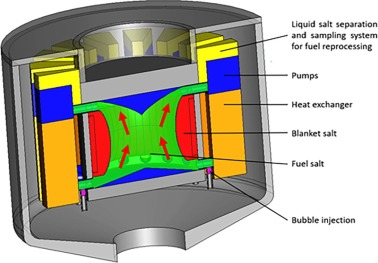
\includegraphics[width=0.48\textwidth]{./figures/MSFR}
	\caption{MSFR reactor design concept \cite{serp_molten_2014}.}
	\label{fig:msfr}
\end{figure} 

\begin{table}[t]
	\caption{Specifications of the \gls{MSFR} design \cite{serp_molten_2014}.}
	\begin{tabular}{ l l }
		\hline
		Parameter & Value \\
		\hline
		Thermal/Electric output [MW$_{\text{th}}$/MW$_{\text{e}}$] & 3000 /
		1500 
		\\
		Salt volume [m$^3$] & 18 \\
		Salt fraction in core & 0.5 \\
		Number of circulation loops & 16 \\
		Nominal flow rate [kg s$^{-1}$] & 18500  \\
		Nominal circulation time [s] & 4.0 \\
		Inlet/outlet temperature [K] & 923 / 1023 \\
		Blanket volume [m$^3$] & 7.3\\
		\hline
	\end{tabular}
	\label{table:msfr}
\end{table}

	The primary fuel salt flows upwards through the 9 m$^3$ central core
	region. At the top of the core, the flow separates into 16 smaller external
	loops, each of which passes through a heat exchanger and is pumped back
	into the core. The primary heat exchangers transfer heat from the fuel salt 
	to an intermediate salt coolant loop. There are other instrumentation along
	the external loops for online reprocessing and gas sparging. The core is
	radially surrounded by a tank of blanket molten salt, with reflectors at
	the top and bottom of the core. The blanket salt contains fertile isotopes
	such as $^{232}$Th for fuel breeding. There is a layer of neutron absorbing
	material behind the blanket tanks to protect the heat exchangers, pumps and
	other instrumentation from neutron irradiation damage.

	Various authors have performed a number of steady state and transient
	multiphysics simulations for the \gls{MSFR}. A paper by Fiorina et al.
	\cite{fiorina_modelling_2014} compares results between coupled models
	developed on the multiphysics code COMSOL and an in-house code developed at
	Delft University of Technology. The models used 2D axisymmetric models of
	the \gls{MSFR} and solved multi-group neutron diffusion equations for the
	neutronics, and they showed good agreement for some of the transient cases
	studied. A more comprehensive 3D model has been developed and studied by
	Aufiero et al. \cite{aufiero_development_2014} using the computional fluid
	dynamics (CFD) toolbox OpenFOAM. Although this model relied on the one
	group neutron diffusion equation, it enabled the study of the full 3D core
	geometry and 3D transient scenarios such as the failure of one of the 16
	pumps in the \gls{MSFR}.

	More recently, a coupled tool, comprising of the thermal-hydraulics code
	TRACE and a multi-group 3D spatial neutronics solver \gls{PARCS}, was
	used to run steady state and transient simulations of the \gls{MSFR}
	\cite{pettersen_coupled_2016}. This approach allowed for a 3D model
	simulation of the \gls{MSFR} on a coarse mesh, thus improving on the 2D
	axisymmetric COMSOL/TUDelft models with the benefit of much lower
	computation times in comparison to the CFD-OpenFOAM models. On top of
	steady state simulations, the transient scenarios studied by Pettersen
	\cite{pettersen_coupled_2016} include loss of heat sink, pump over-speed,
	over-cooling and loss of flow.

\section{Methodology}

	This section describes the overall modelling approach and the codes used
	in this paper. First, the \gls{BOL} and equilibrium compositions were
	obtained from SCALE/TRITON unit cell depletion calculations by Rykhlevskii
	et al. (cite Andrei) Their paper used a unit cell model for the modelling
	fuel cycle performance of the \gls{MSFR} and three other fast-spectrum
	\glspl{MSR}. The neutron spectrum and depletion calculations on the unit
	cell SCALE/TRITON models were verified against full core SERPENT models and
	showed very good agreement. The equilibrium composition was selected at
	approximately 43 years after start-up because the TRU vector change
	between each depletion time-step from this moment onwards is less than 3\%.
	(cite Andrei) For the \gls{BOL} composition, it is the fuel composition at
	300 days after start-up. Decay isotopes, whose neutron cross-section data
	are not found in the
	JEFF-3.1.2 nuclear data library, were omitted.
	
	Neutronics calculations were performed on SERPENT using these fuel
	compositions and a truncated, reference \gls{MSFR} core model
	\cite{pettersen_coupled_2016} to generate six-group neutronics data for
	Moltres.
	The energy boundaries for the six neutron groups are adopted from previous
	\gls{MSFR} studies and shown in Table \ref{table:bound}.
	As for the \gls{DNP} groups, there are eight groups as defined by the
	JEFF-3.1.2 nuclear data library used for neutron cross-section data.
	The reactor model is a 2D axisymmetric model as shown in
	Figure \ref{fig:reference}. This geometry focuses on the active central
	region of the core. Basing the geometry on the reference model facilitates
	comparisons with previous MSFR studies by various authors
	\cite{fiorina_modelling_2014} \cite{pettersen_coupled_2016} on the
	reference model for code-to-code verification purposes.
	The 2D model is extended into a 3D model in SERPENT by rotating it
	around the central axis to form concentric cylinders.
	
\begin{table}[b]
	\centering
	\captionsetup{justification=centering}
	\caption{Neutron energy group upper bounds used in Serpent.}
	\begin{tabular}{ll}
		\hline
		{Group number} & {Upper bound [MeV]}\\
		\hline
		1 & 7.485$\times 10^{-4}$\\
		2 & 5.5308$\times 10^{-3}$\\
		3 & 2.47875$\times 10^{-2}$\\
		4 & 0.4979\\
		5 & 2.2313\\
		6 & 12\\
		\hline
	\end{tabular}
	\label{table:bound}
\end{table}	
	
	Finally, with the group constant data from SERPENT, Moltres
	calculated the resulting coupled neutron spectrum and temperature
	distribution for a given velocity profile in the core, from user-specified
	initial conditions towards steady state, or from steady state in the case
	of an accident scenario. The mesh geometry for Moltres is
	further simplified from the SERPENT model by the omission of the absorber,
	heat exchanger, and reflector regions. This is justified as they have
	negligible contribution towards the neutronics. Instead, a vacuum
	boundary condition was imposed on the outer surface of the blanket region,
	along with 923 K Dirichlet boundary conditions for temperature.
	The 2 cm thick blanket tank structural material was also omitted as its
	inclusion resulted in an extra fine mesh which drastically
	increased computational time. (Insert Moltres mesh model)
	
	Moltres has a loop app functionality to account for the flow and decay of
	\glspl{DNP} outside the active core region. For this paper, the two ends of
	a separate, 188 cm long 1-D outer
	loop region were ``attached" to the inlet and outlet of active core region
	model, shown in Figure *, to form a closed coolant loop. This was achieved
	using \gls{DNP} boundary
	conditions at the inlets and outlets of the core and outer loop geometry,
	determined by the inflow and outflow values of each \gls{DNP} group at
	each time-step for each boundary.
	\gls{DNP} in the outer loop are also governed by the same \gls{DNP}
	equations to allow for flow, production, and decay.
	
	The velocity profile is a uniform velocity of $1.1275$ ms$^{-1}$ throughout
	the active core and outer loop regions. This value is derived from the
	\gls{MSFR} loop circulation time of 4 s. Moltres also has a heat exchanger
	kernel defined for simulating heat loss through
	a heat exchanger. For this paper, the kernel was placed at the midpoint of
	the outer loop region, with the heat loss value fixed to induce an
	approximately 100 K
	drop in temperature as specified by the \gls{MSFR} design inlet/outlet
	temperature difference.
	
	
\begin{figure}[t] 
	\centering
	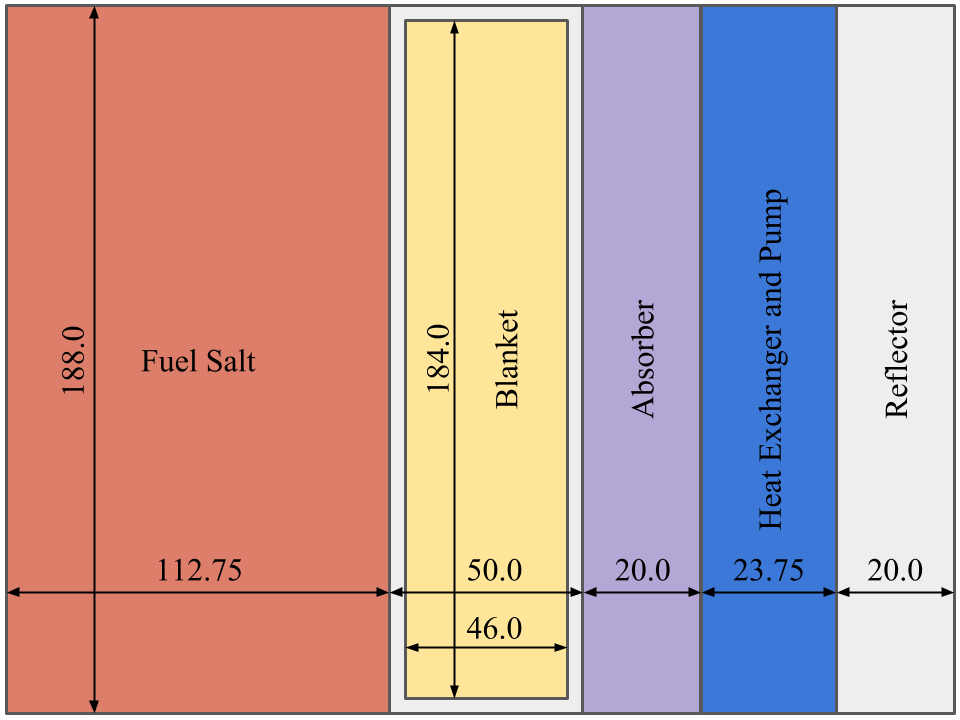
\includegraphics[width=0.46\textwidth]{./figures/reference}
	\captionsetup{justification=centering}
	\caption{Cross-section of the 2D axisymmetric model used for the
	simulation. Derived from the 2D axisymmetric reference model of the MSFR
	\cite{pettersen_coupled_2016}. The figure is not drawn to scale.}
	\label{fig:reference}
\end{figure} 

\subsection{\textbf{Moltres Code}}

	This subsection provides the theoretical background for the coupled
	neutronics/thermal-hydraulics physics implemented in Moltres.
	
	Moltres is an application code developed in the \gls{MOOSE} framework
	\cite{gaston_moose:_2009}. \gls{MOOSE} application codes solve non-linear
	problems through the discretization of \glspl{PDE} on an adaptive coarse
	meshing scheme provided by LibMesh \cite{kirk_libmesh:_2006} and PetSc
	\cite{satish_balay_petsc_2015}. Individual terms of \glspl{PDE} that define
	the physics involved in a system are represented in \gls{MOOSE} (and its
	applications) by kernels. For example, the various terms in the neutron
	diffusion equation such as the diffusion term, time evolution term, etc.
	all have a corresponding physics kernel defined in Moltres. Boundary
	conditions are also handled in a similar fashion. Moltres can solve for an
	arbitrary number of neutronics groups as long as the relevant group
	constants are provided in a Moltres-compatible format.

	As mentioned in the previous Moltres study
	\cite{lindsay_introduction_2018}, the neutronics in Moltres is described by
	the time-independent multi-group neutron diffusion equation as shown in
	Equation \ref{eq1}:
%
\begin{align}
	\frac{1}{v_g} &\frac{\partial \phi_g}{\partial t} - \nabla \cdot D_g \nabla
	\phi_g + \Sigma^r_g \phi_g \nonumber \\ 
	&= \sum^G_{g \neq g'} \Sigma^s_{g' \rightarrow g} \phi_{g'} + \chi^p_g
	\sum^G_{g'=1} (1-\beta) \nu \Sigma^f_{g'} \phi_{g'} + \chi^d_g \sum^I_i
	\lambda_i C_i, \label{eq1}
\end{align}
%
	where

{
\small
\begin{align}
	v_g &= \text{average speed of neutrons in group }g \\
	\phi_g &= \text{flux of neutrons in group }g \\
	t &= \text{time} \\
	D_g &= \text{diffusion coefficient of neutrons in group }g \\
	\Sigma^r_g &= \text{macroscopic cross-section for removal of neutrons} 
	\nonumber \\
	&\text{from group }g \\
	\Sigma^s_{g' \rightarrow g} &= \text{macroscopic cross-section of
	scattering from }g' \text{ to }g \\
	\chi^p_g &= \text{prompt fission spectrum neutrons in group }g \\
	G &= \text{number of discrete neutron groups, }g \\
	\nu &= \text{average number of neutrons produced per fission} \\
	\Sigma^f_{g} &= \text{macroscopic fission cross-section} \nonumber \\
	&\text{for neutron in group }g \\
	\chi^d_g &= \text{delayed fission spectrum neutrons in group }g \\
	I &= \text{number of delayed neutron precursor groups} \\
	\beta &= \text{delayed neutron fraction} \\
	\lambda_i &= \text{average decay constant of delayed neutron} \nonumber \\
	&\text{precursors in precursor group }i \\
	C_i &= \text{concentration of delayed neutron precursors} \nonumber \\
	&\text{in precursor group }i .
\end{align}
}

	The \glspl{DNP} are governed by the following equation:
%
\begin{align}
	\frac{\partial C_i}{\partial t} = \sum^G_{g'=1} \beta_i \nu \Sigma^f_{g'}
	\phi_{g'} - \lambda_i C_i - \frac{\partial}{\partial z} u C_i. \label{eq2}
\end{align}

	Lastly, the governing equation for temperature in the molten salt is given
	as:
%
\begin{align}
	\rho c_{p} \frac{\partial T}{\partial t} + \nabla \cdot \big( \rho
	c_{p} \overrightarrow{u} \cdot T - k \nabla T \big) = Q,
	\label{eq3}
\end{align}
%
	where
{\small
\begin{align}
	\rho &= \text{density of molten salt} \\
	 c_{p} &= \text{specific heat capacity of molten salt} \\
	 T &= \text{temperature of molten salt} \\
	 \overrightarrow{u} &= \text{velocity of molten salt} \\
	 k &= \text{thermal conductivity of molten salt},
\end{align}
}
	and the source term $Q$ is given as:
%
\begin{align}
Q = \sum^G_{g=1} \epsilon_g \Sigma_g^f \phi_g. \label{eq4}
\end{align}

\section{Steady State Neutron Flux and Temperature Distribution}

	The \gls{MSFR} Moltres simulations were run in transient mode, with
	adaptive time-stepping, and with an
	initial neutron flux of $10^{14}$
	\# cm$^{-2}$ s$^{-1}$ and an initial temperature of 923 K throughout the
	fuel and blanket regions, for the start-up, \gls{BOL}, and equilibrium
	fuel compositions. The simulations reached steady state after 100 s, as the
	volume-integrated neutron flux values varied by less than 0.001\% over the
	last ten seconds. The computational time for each case averages at 30
	minutes when run on four cores on a workstation.
	
	Figure \ref{fig:totalflux} shows the total radial neutron flux at reactor
	half-height, with the three fuel compositions at steady state. 
	The peak neutron flux value is highest for the start-up composition,
	followed by the \gls{BOL} and equilibrium compositions. All three values
	are slightly lower than the peak value of approximately
	$8.6 \times 10^{15}$ \# cm$^{-2}$ s$^{-1}$ reported by Fiorina et al.
	\cite{fiorina_investigation_2013}. This may be due to the truncation of
	the top and bottom fuel regions of the core for the model used here.
	The vacuum boundary conditions were imposed closer to the center and
	resulted in a lower peak value. Figure \ref{fig:stflux} shows the six
	neutron group fluxes for the start-up fuel composition.
	
	Heat transfer is dominated by advection as is observed by the temperature
	distributions in Figure \ref{fig:temp}. Given that flux is the highest
	at the center of the core, most of the heat is produced there. The upward
	flow pushes the temperature peak up to the outlet boundary. Tables
	\ref{table:inlet} and \ref{table:outlet} show the average
	fuel inlet and outlet temperatures for the three cases.
%	
\begin{table}[H]
	\centering
	\captionsetup{justification=centering}
	\caption{Average fuel inlet temperature.}
	\begin{tabular}{ll}
		\hline
		{Composition} & {Inlet temperature [K]}\\
		\hline
		Start-up & 964.85\\
		\gls{BOL} & 925.11\\
		Equilibrium & 916.85\\
		\hline
	\end{tabular}
	\label{table:inlet}
\end{table}	
%
\begin{table}[H]
	\centering
	\captionsetup{justification=centering}
	\caption{Average fuel outlet temperature.}
	\begin{tabular}{ll}
		\hline
		{Composition} & {Outlet temperature [K]}\\
		\hline
		Start-up & 1067.40\\
		\gls{BOL} & 1025.39\\
		Equilibrium & 1016.67\\
		\hline
	\end{tabular}
	\label{table:outlet}
\end{table}	

\begin{figure*}%
\centering
\begin{subfigure}{1\columnwidth}
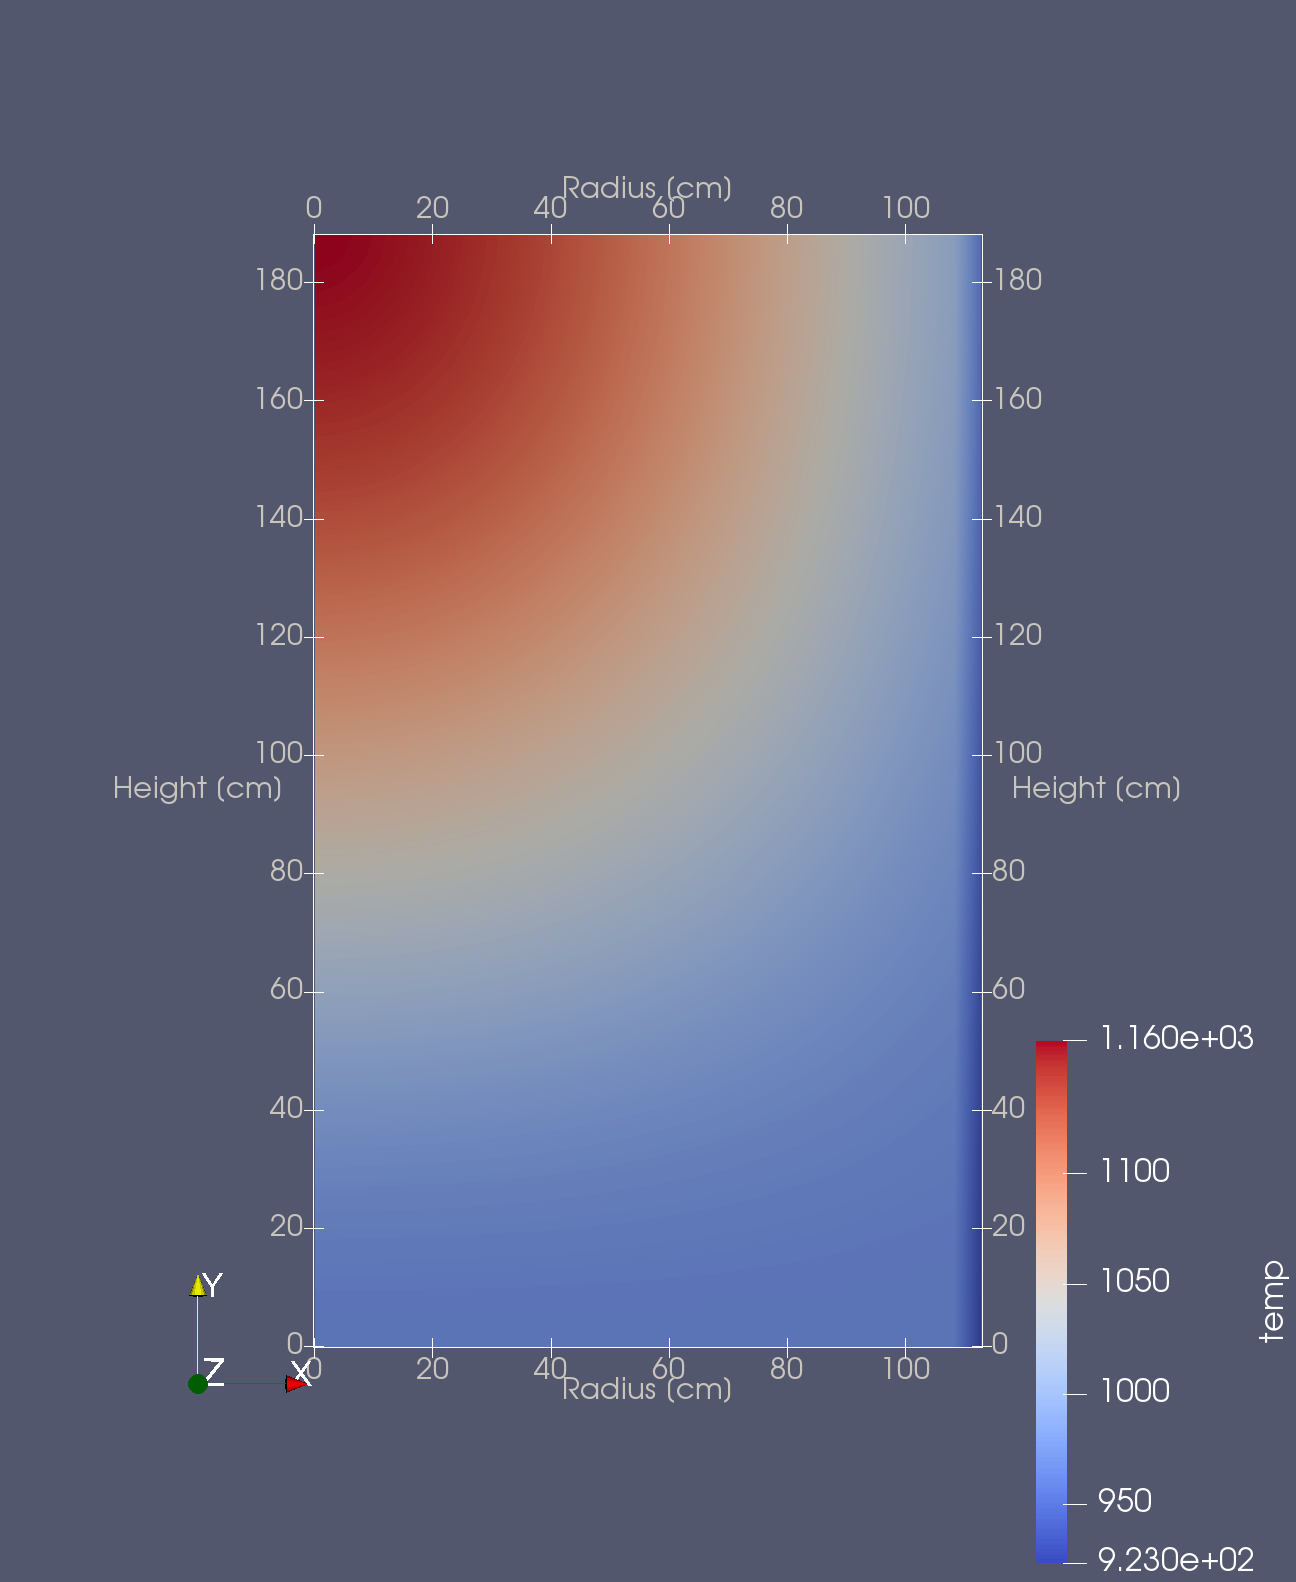
\includegraphics[width=\columnwidth]{./figures/sttemp}%
\end{subfigure}\hfill%
\begin{subfigure}{1\columnwidth}
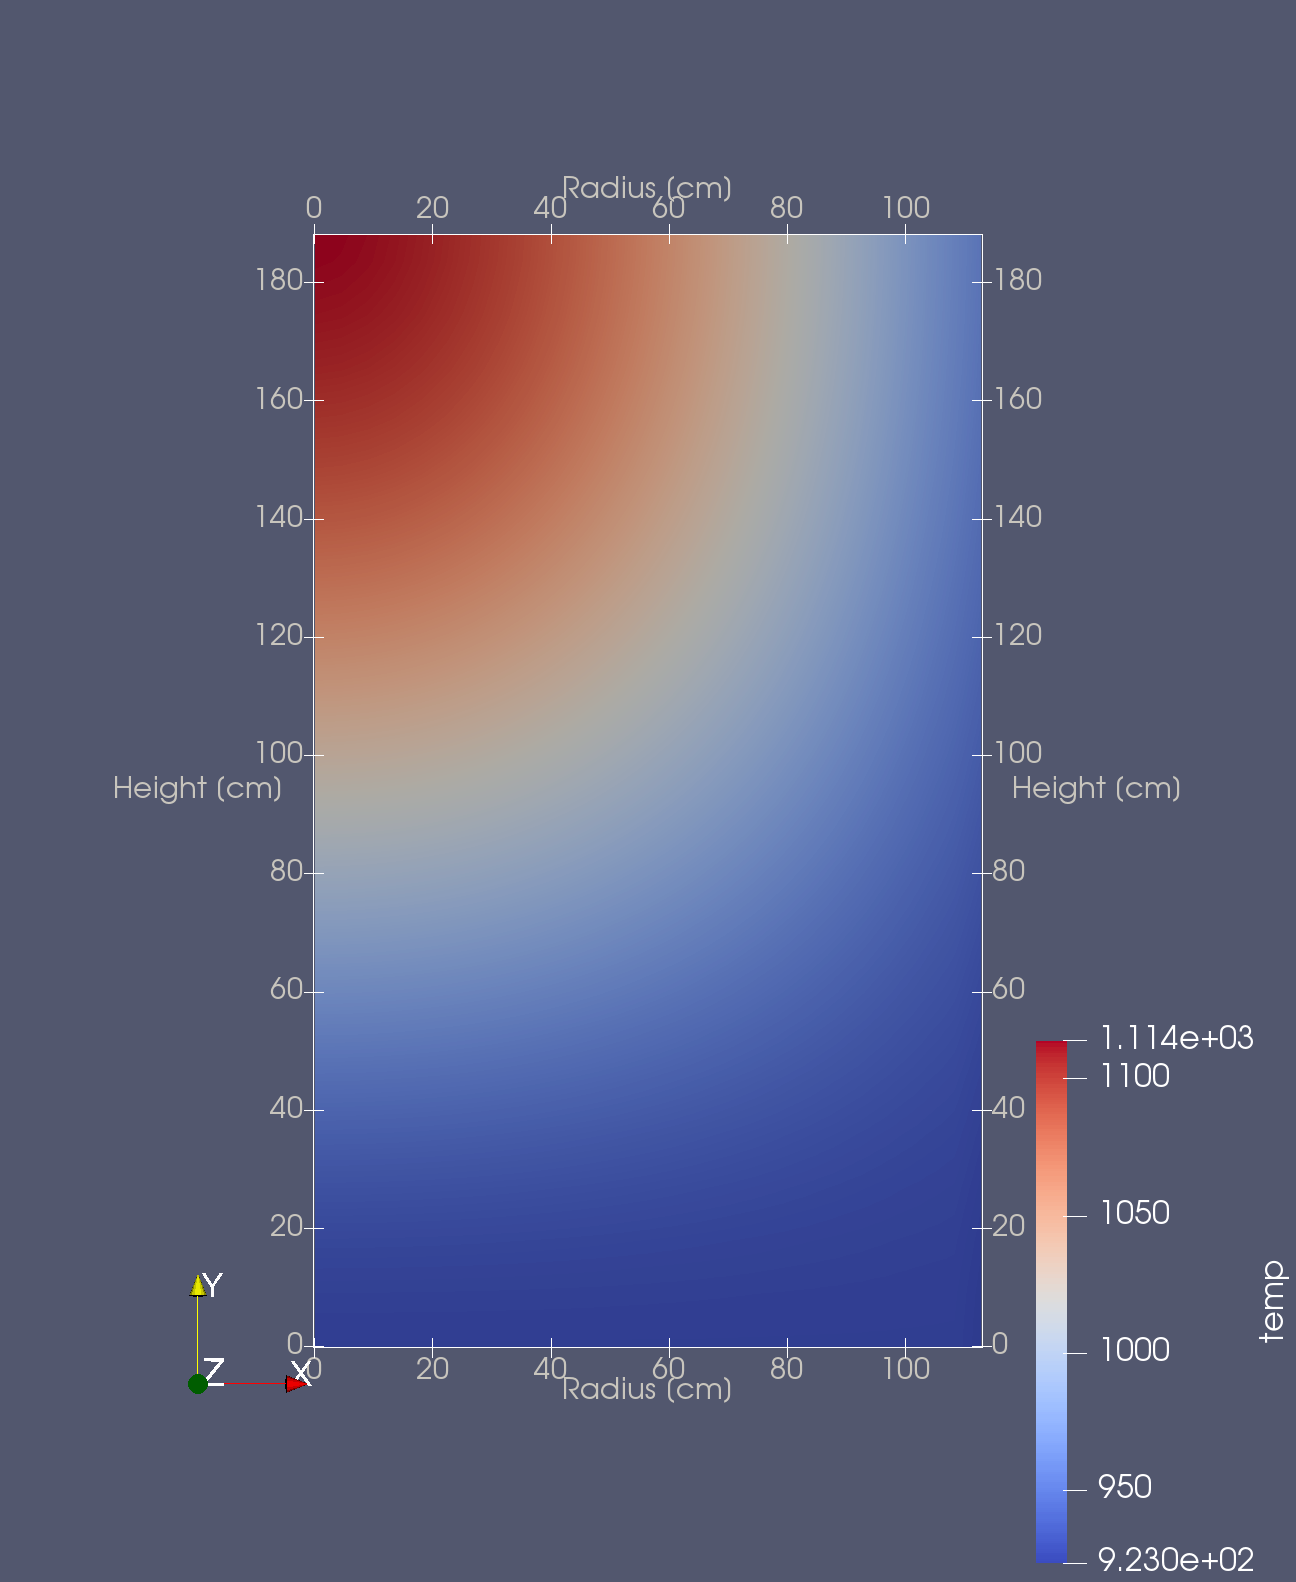
\includegraphics[width=\columnwidth]{./figures/eltemp}%
\end{subfigure}\hfill\\
\bigskip
\centering
\begin{subfigure}{1\columnwidth}
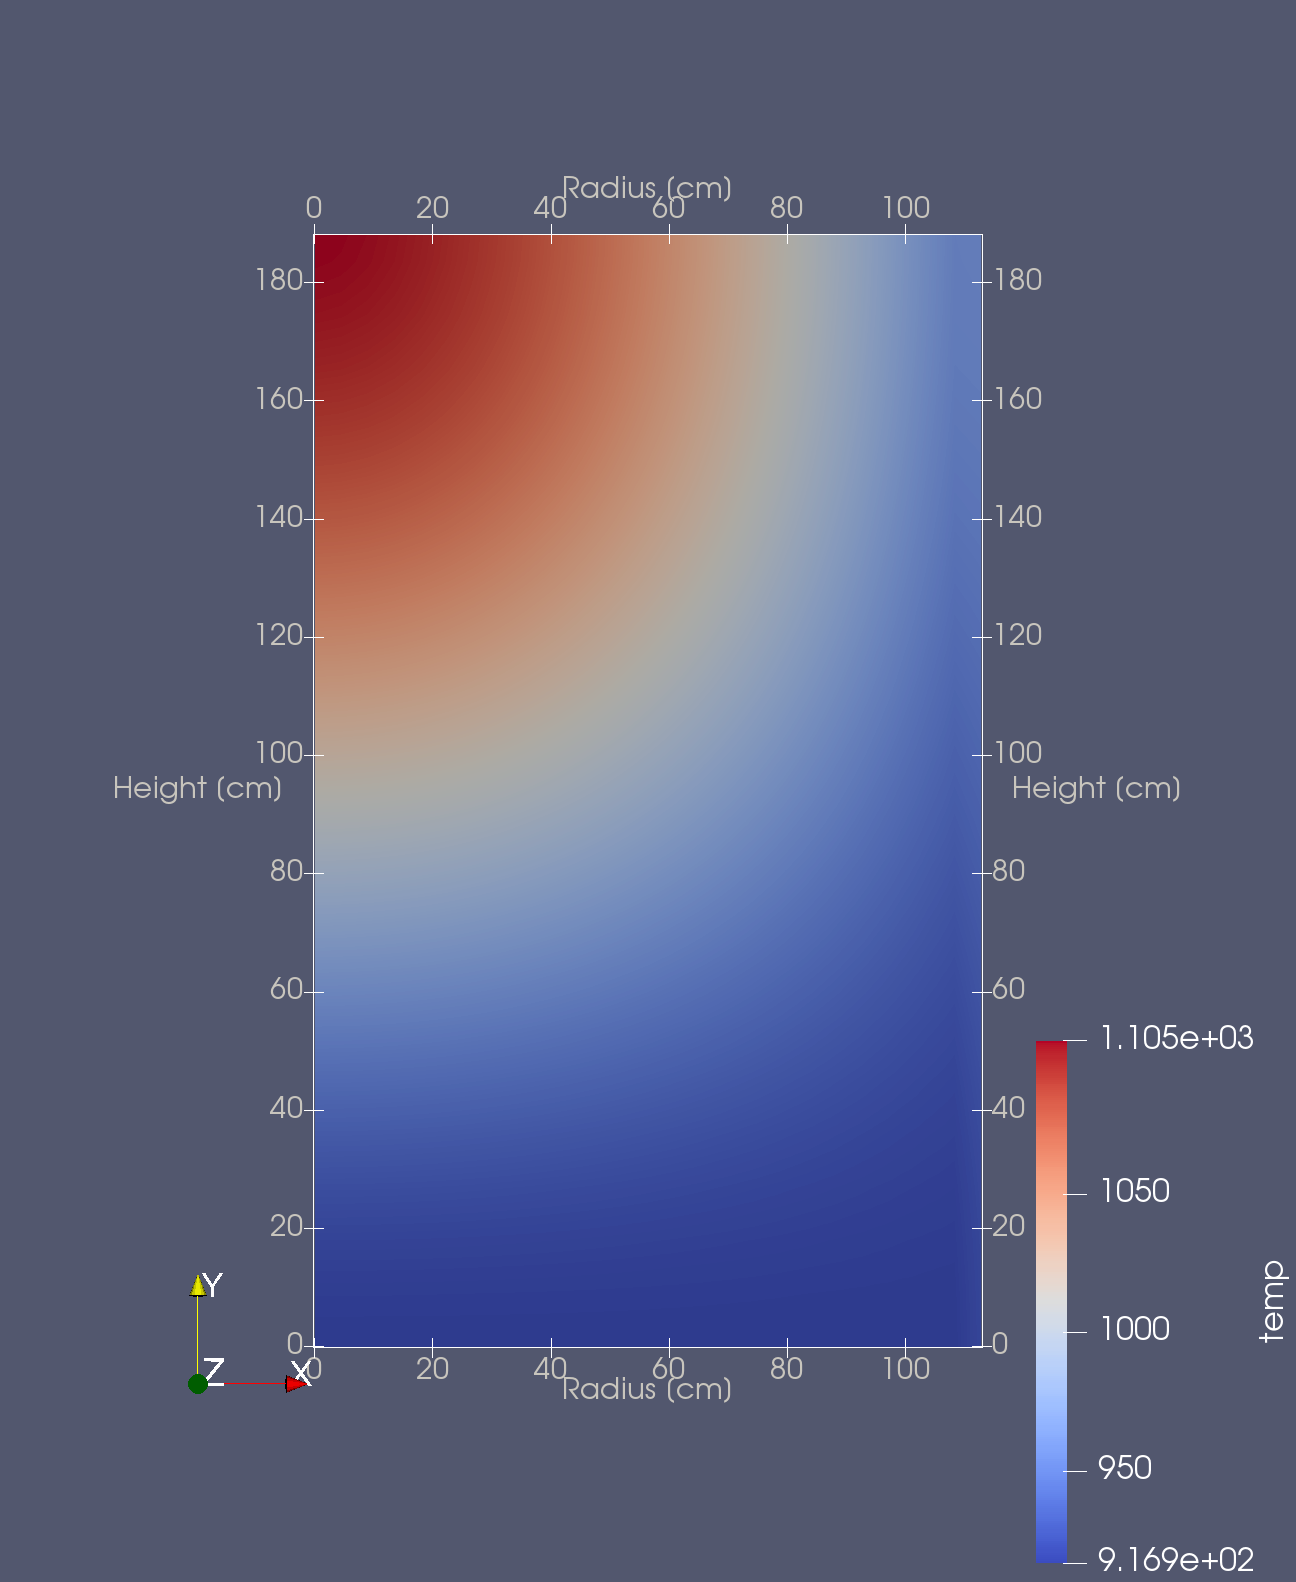
\includegraphics[width=\columnwidth]{./figures/eqtemp}%
\label{subfigc}%
\end{subfigure}%
\captionsetup{justification=centering}
\caption{Temperature distributions within the fuel salt region, for start-up
(top left), \gls{BOL} (top right), and equilibrium (bottom) fuel compositions at steady state. The height and radius are in the Y and X directions
respectively.}
\label{fig:temp}
\end{figure*}
%
\begin{figure}[H] 
	\centering
	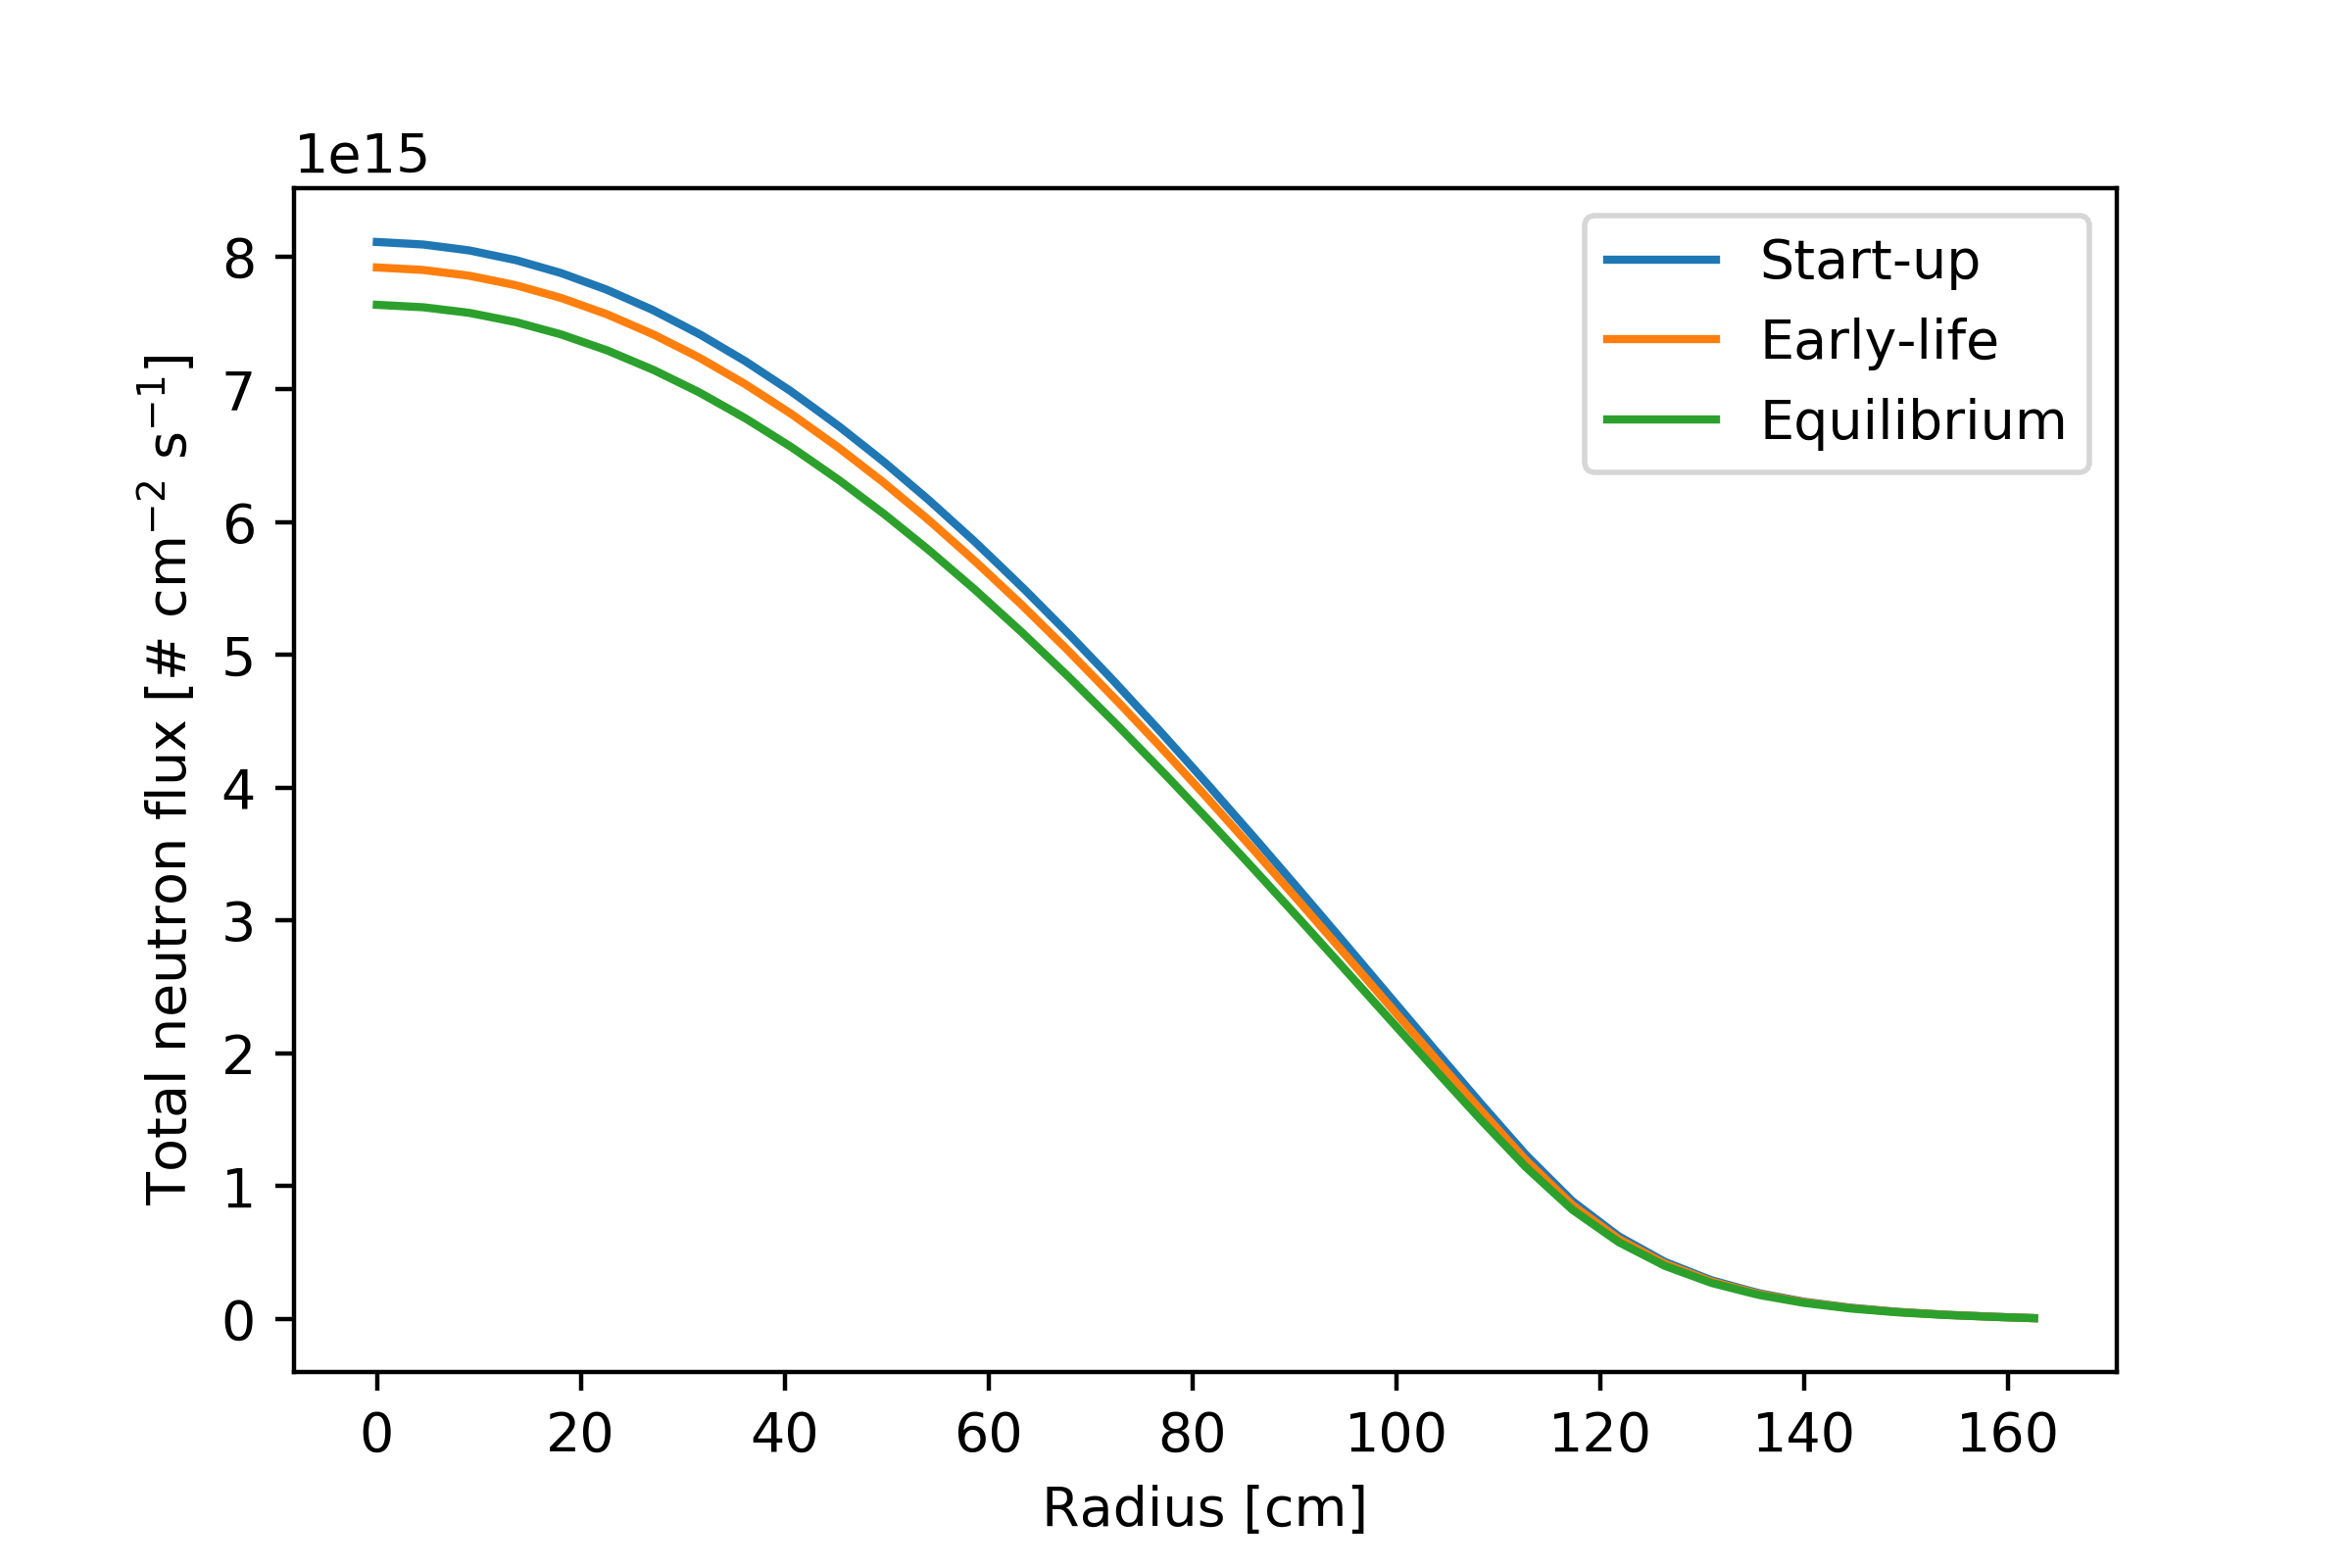
\includegraphics[width=.53\textwidth]{./figures/totalflux}
	\captionsetup{justification=centering}
	\caption{Total radial neutron flux at reactor half-height, for start-up,
	\gls{BOL}, and equilibrium fuel compositions at steady state.}
	\label{fig:totalflux}
\end{figure} 
\begin{figure}[H] 
	\centering
	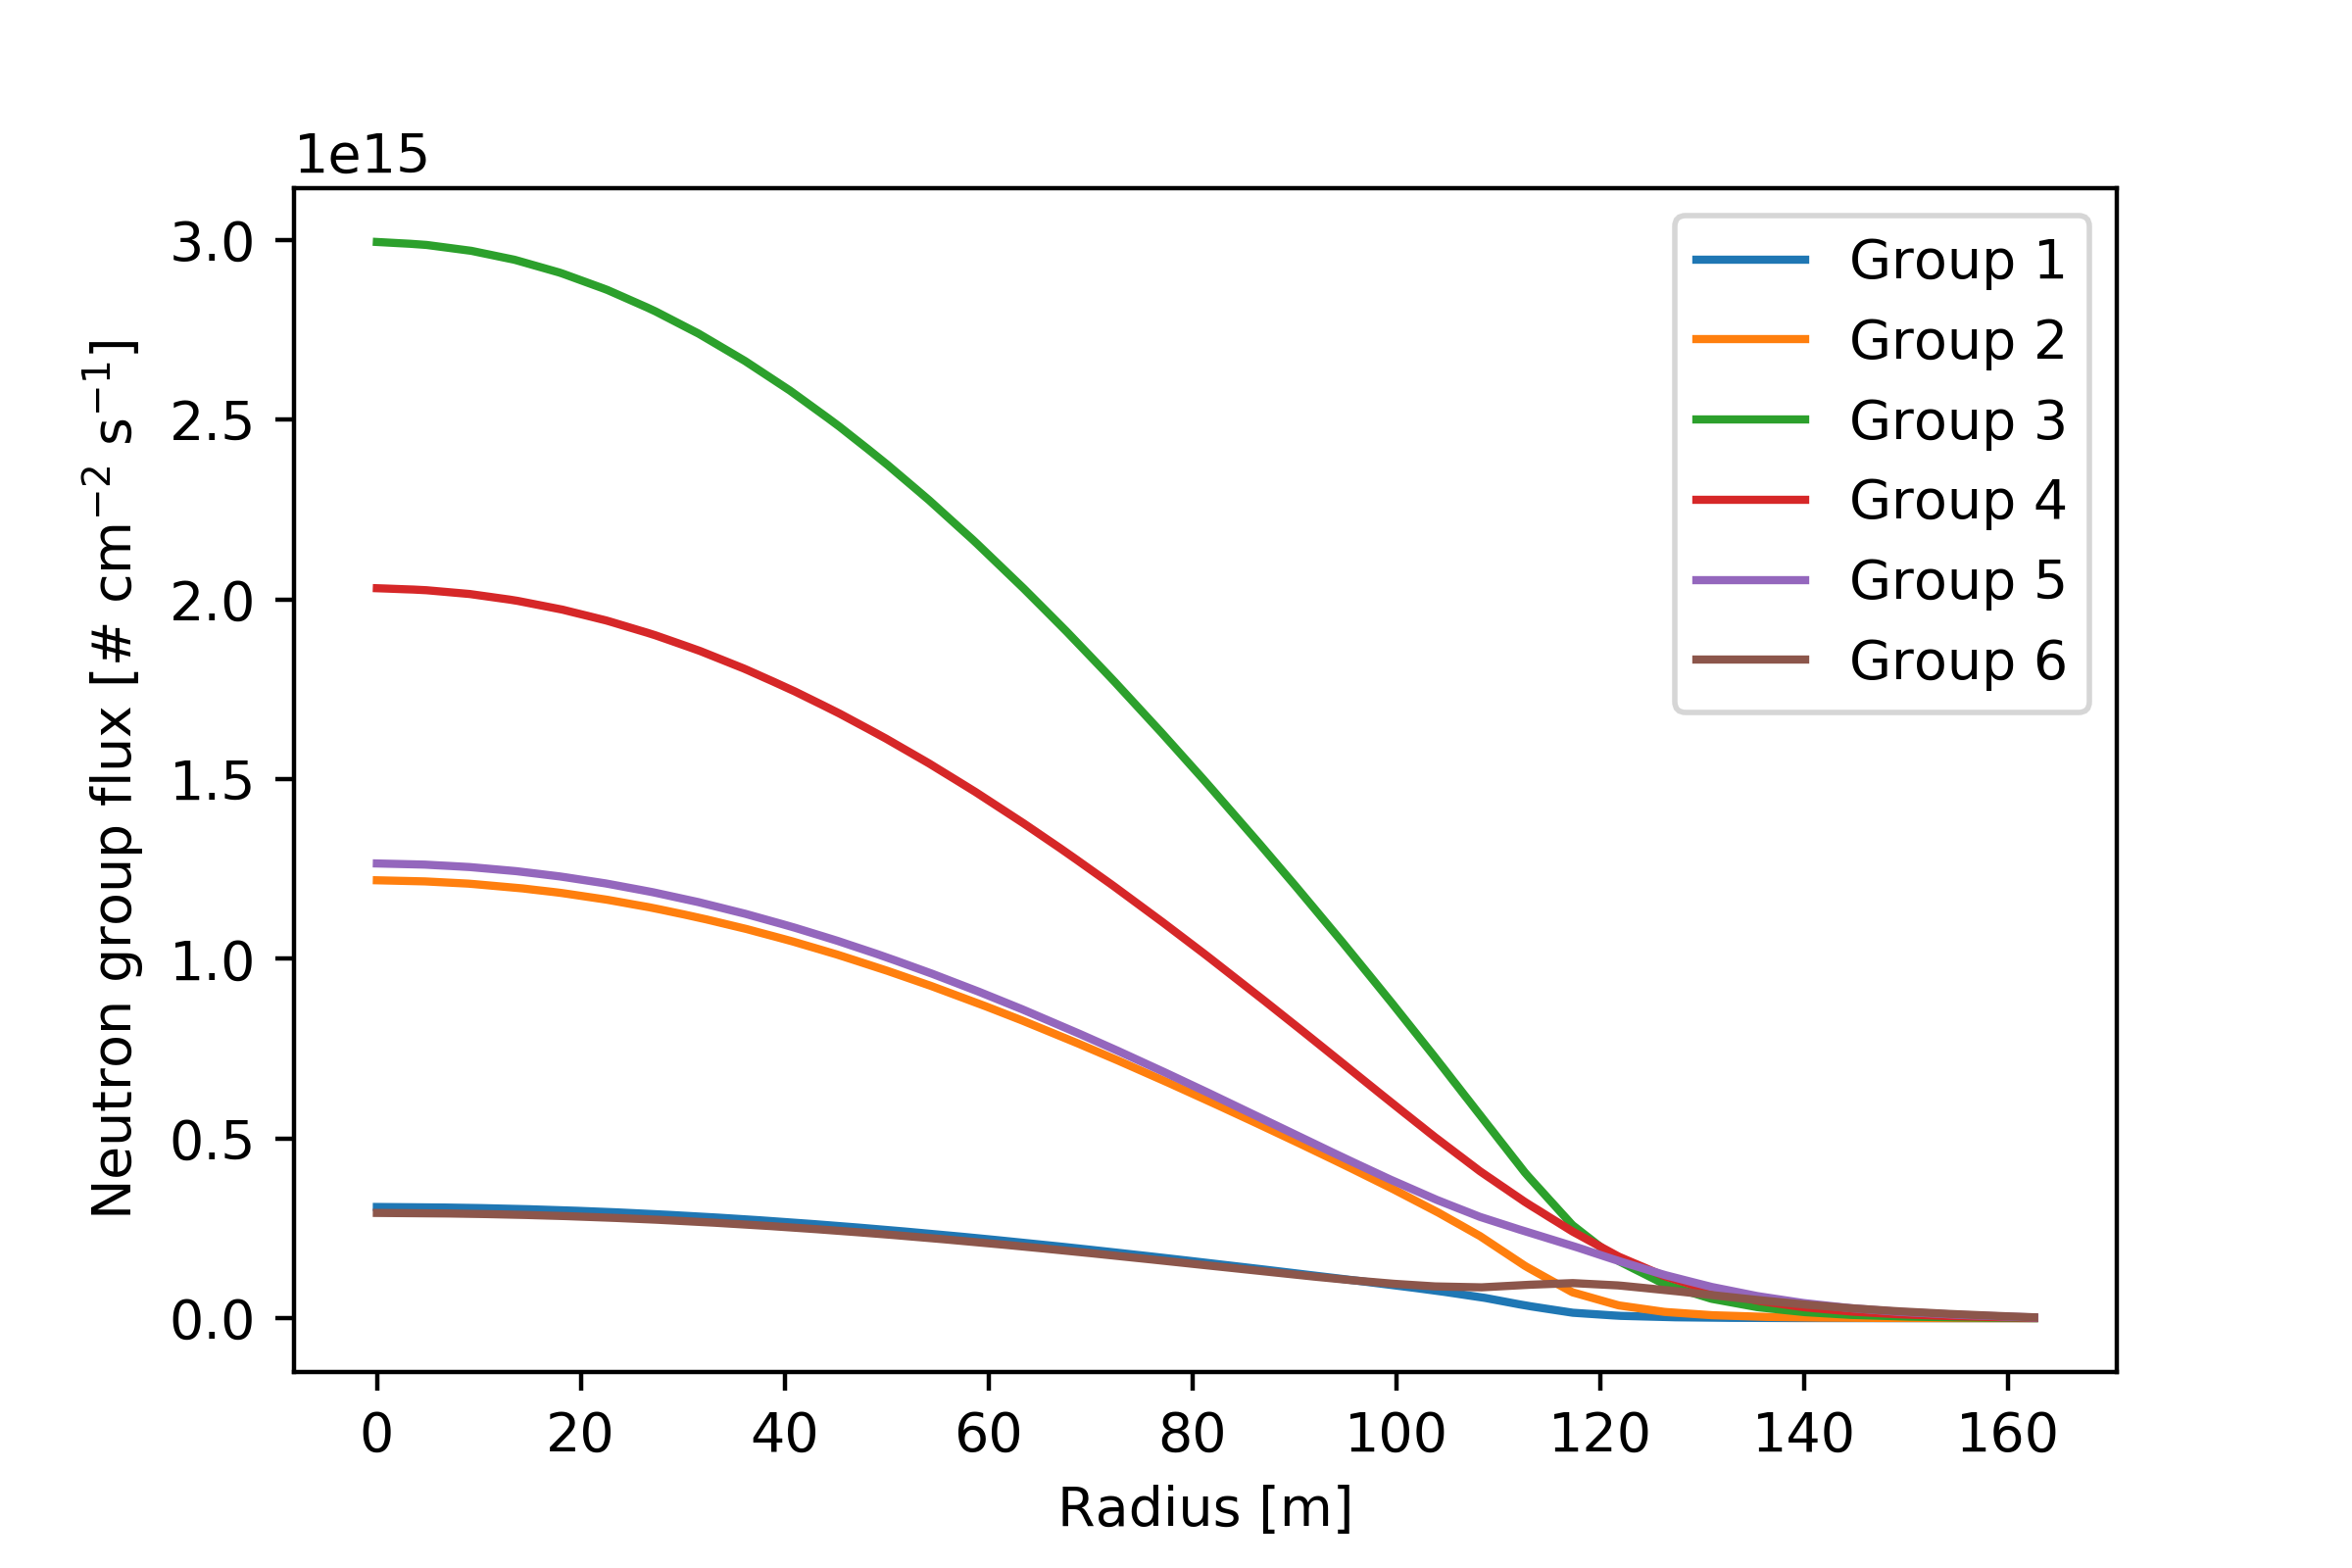
\includegraphics[width=.53\textwidth]{./figures/stflux}
	\captionsetup{justification=centering}
	\caption{Neutron group fluxes at reactor half-height, for start-up
	fuel composition at steady state.}
	\label{fig:stflux}
\end{figure} 

	The temperature distribution is very different from the results by Fiorina
	et al. \cite{fiorina_modelling_2014} and Pettersen
	\cite{pettersen_coupled_2016} because we assumed a uniform velocity
	profile. In reality, there is significant flow stagnation in the fuel salt
	near the blanket tank. This causes temperatures to peak near the blanket
	tank as opposed to the center of the core as seen in Figure \ref{fig:temp}.
	However, improved models of the \gls{MSFR}, as shown by Aufiero et al.
	\cite{aufiero_development_2014}, have temperature distributions closer to
	the results in this paper through curved walls that optimize salt flow.
	
	Total power as defined by Eq. \ref{eq4} is approximately 2 GW. This
	is 1 GW less than the rated 3 GW of the \gls{MSFR}. This may be mainly due
	to the erroneous uniform velocity profile imposed in the core. From
	fluid dynamics, velocity along the central axis of the core should be
	higher than the velocity at the periphral areas near the blanket tank.
	The higher velocity at the center results in higher advective heat transfer
	away from the center of the core and cools the active region. This should
	result in an increase in neutron flux from the strongly negative
	temperature reactivity feedback, and thus higher heat generation. The
	truncation of the top and bottom fuel salt region is also a factor for
	the lower than expected heat production.
	
	Comparing the three different fuel compositions, the \gls{MSFR} operates at
	the highest temperatures with the start-up fuel composition, followed by
	the \gls{BOL}, and the equilibrium compositions. This may be due to the
	generation of $^{233}$Pa as an intermediate for $^{233}$U breeding as
	mentioned by Rykhlevskii et al. (cite Andrei) in their fuel cycle analysis
	of the \gls{MSFR}.

\section{Loss of Secondary Cooling Accident}

	A \gls{LOSCA} may occur due to various causes of failure in the secondary
	coolant loop such as secondary loop pump failure or loss of secondary
	coolant. While it is less likely in an \gls{MSFR} as it consists of 16
	separate coolant loops each with its own secondary cooling system, the
	potential consequences must still be studied.
	The loss of secondary cooling is simulated by exponentially decreasing
	the heat loss rate in the Moltres heat exchanger kernel with a time
	constant of 5 s.
	
	The loss of heat sink is expected to cause an initial temperature spike,
	followed by a decrease in neutron flux and heat generation due to the
	strongly negative temperature reactivity feedback. Eventually, the
	\gls{MSFR} should settle on a new steady state with a higher average
	temperature than the operating temperature. If the high temperature is
	sustained for a long period of time, it could lead to severe damage
	in the reactor, pipes, or other instruments.
	
\begin{figure}[b] 
	\centering
	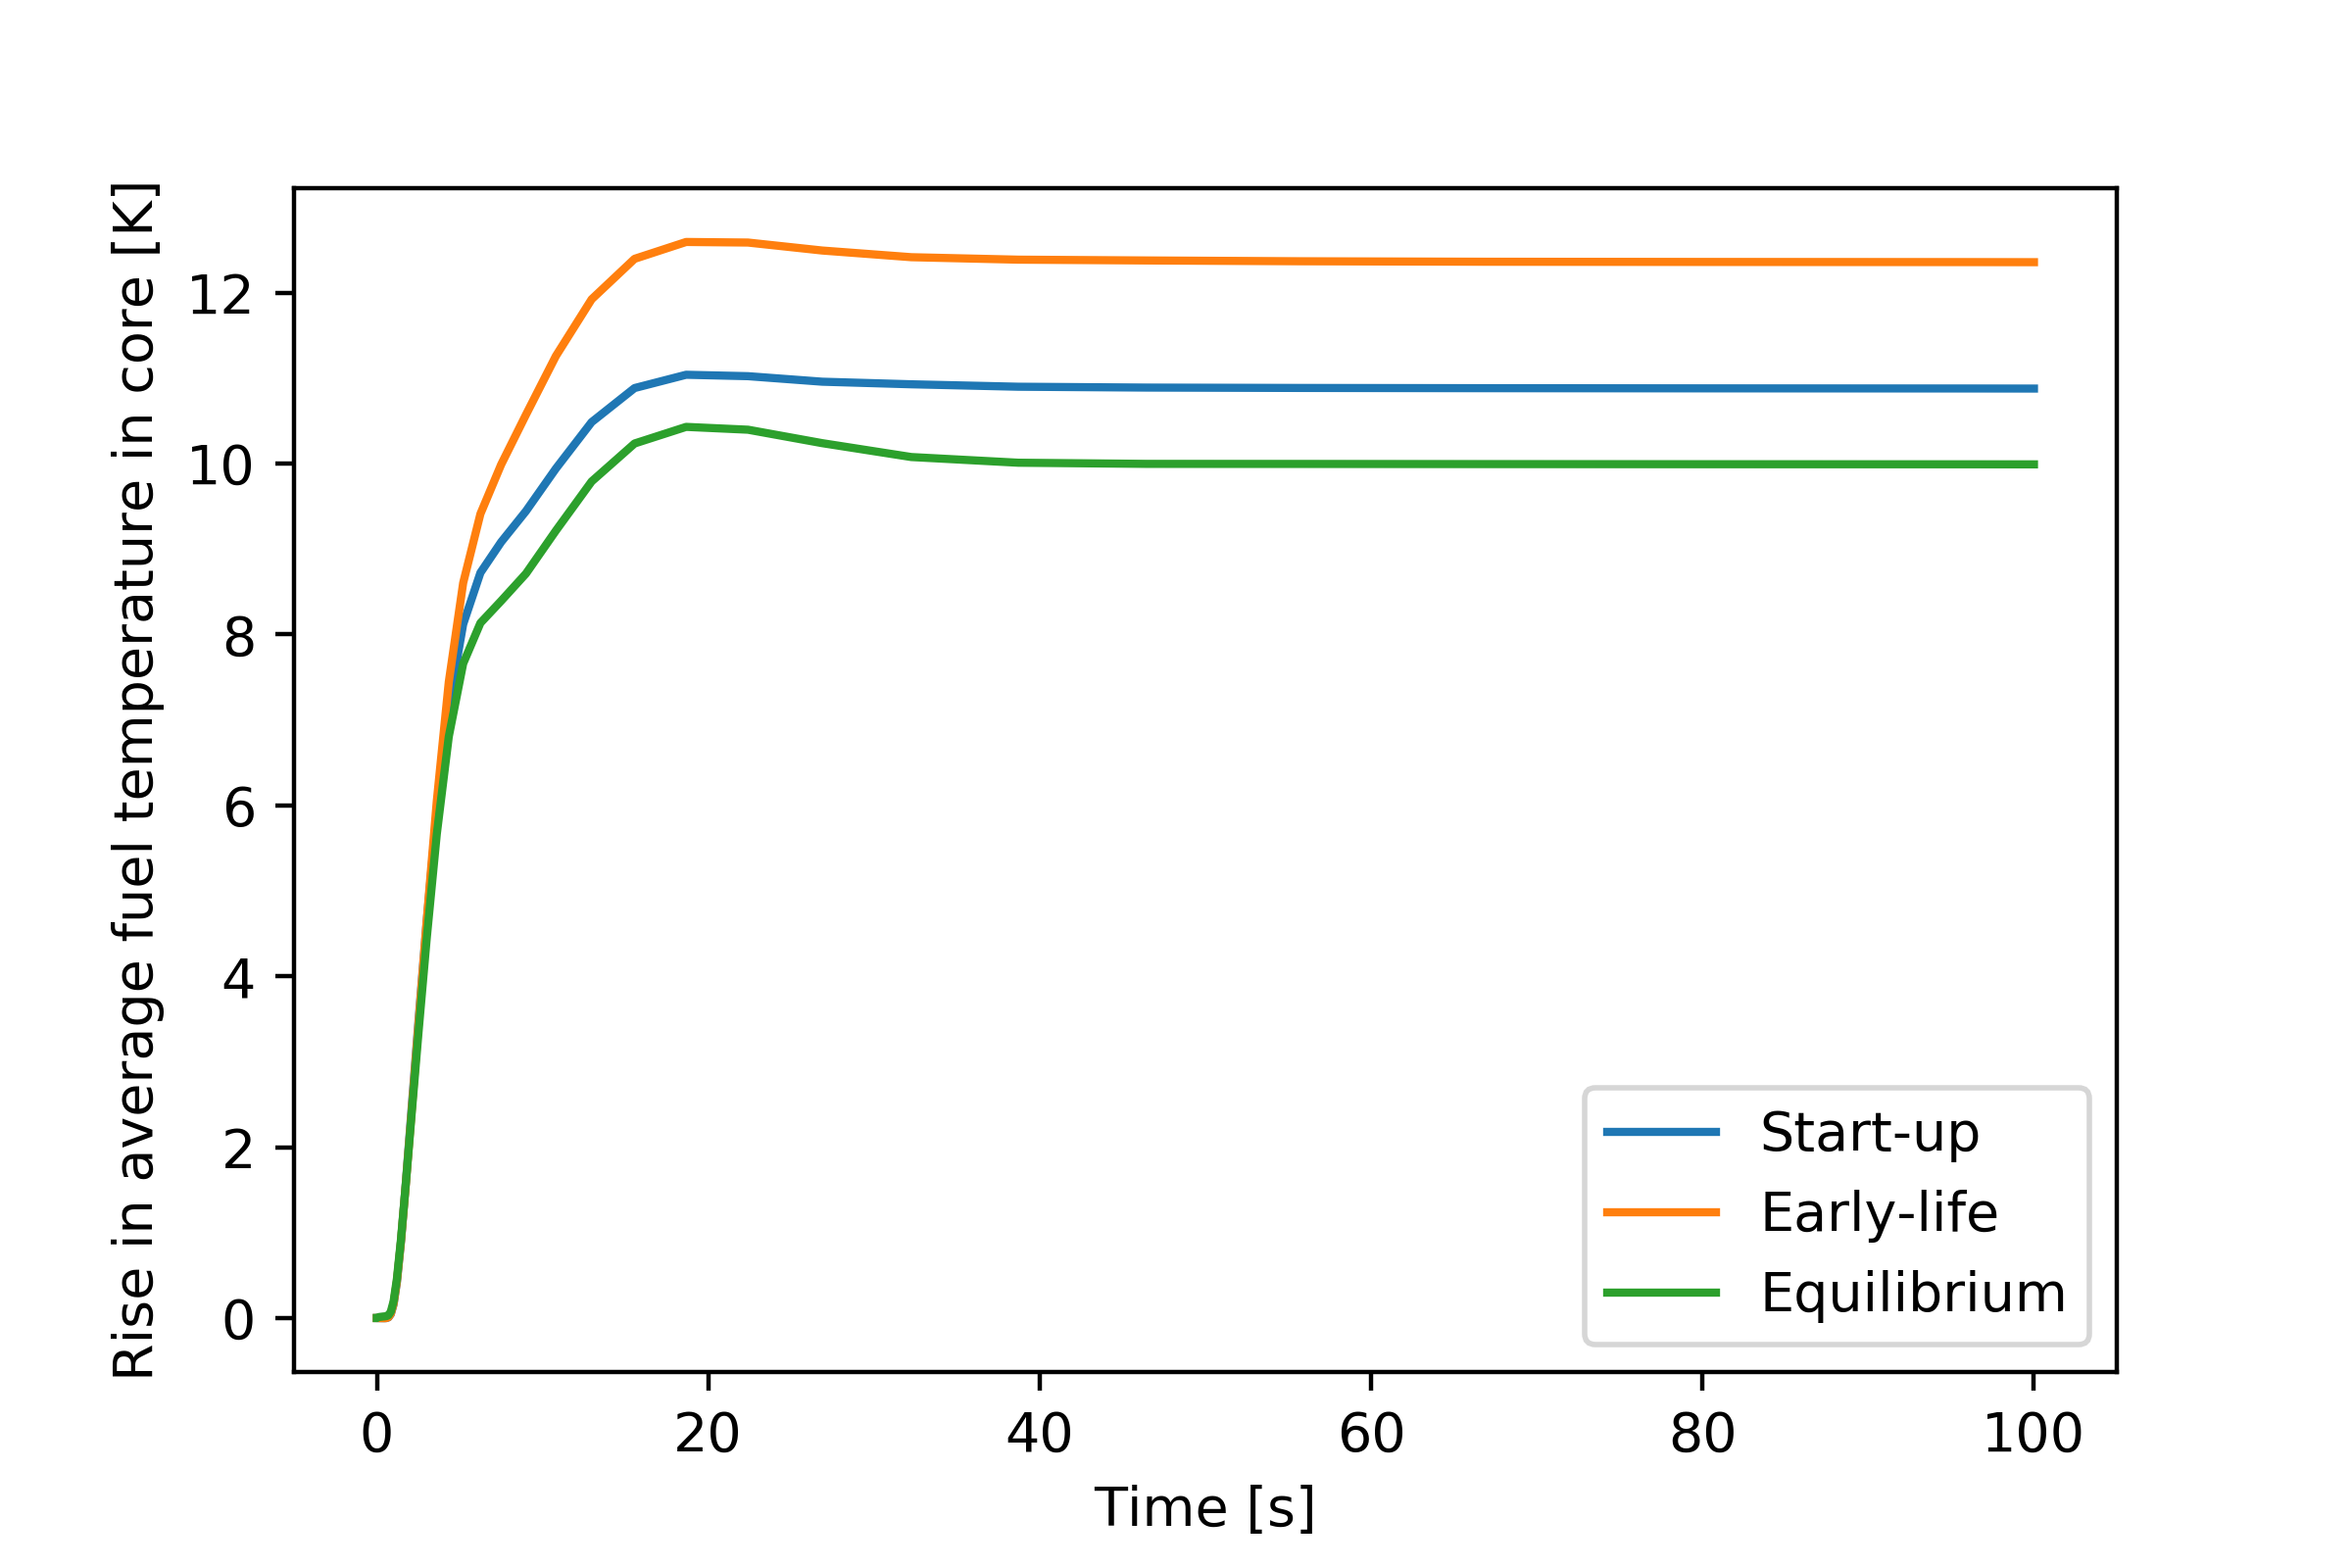
\includegraphics[width=.53\textwidth]{./figures/loscatemp}
	\captionsetup{justification=centering}
	\caption{Average core fuel temperature for start-up, \gls{BOL}, and
	equilibrium fuel compositions during \gls{LOSCA}.}
	\label{fig:loscatemp}
\end{figure} 
%
\begin{figure}[t] 
	\centering
	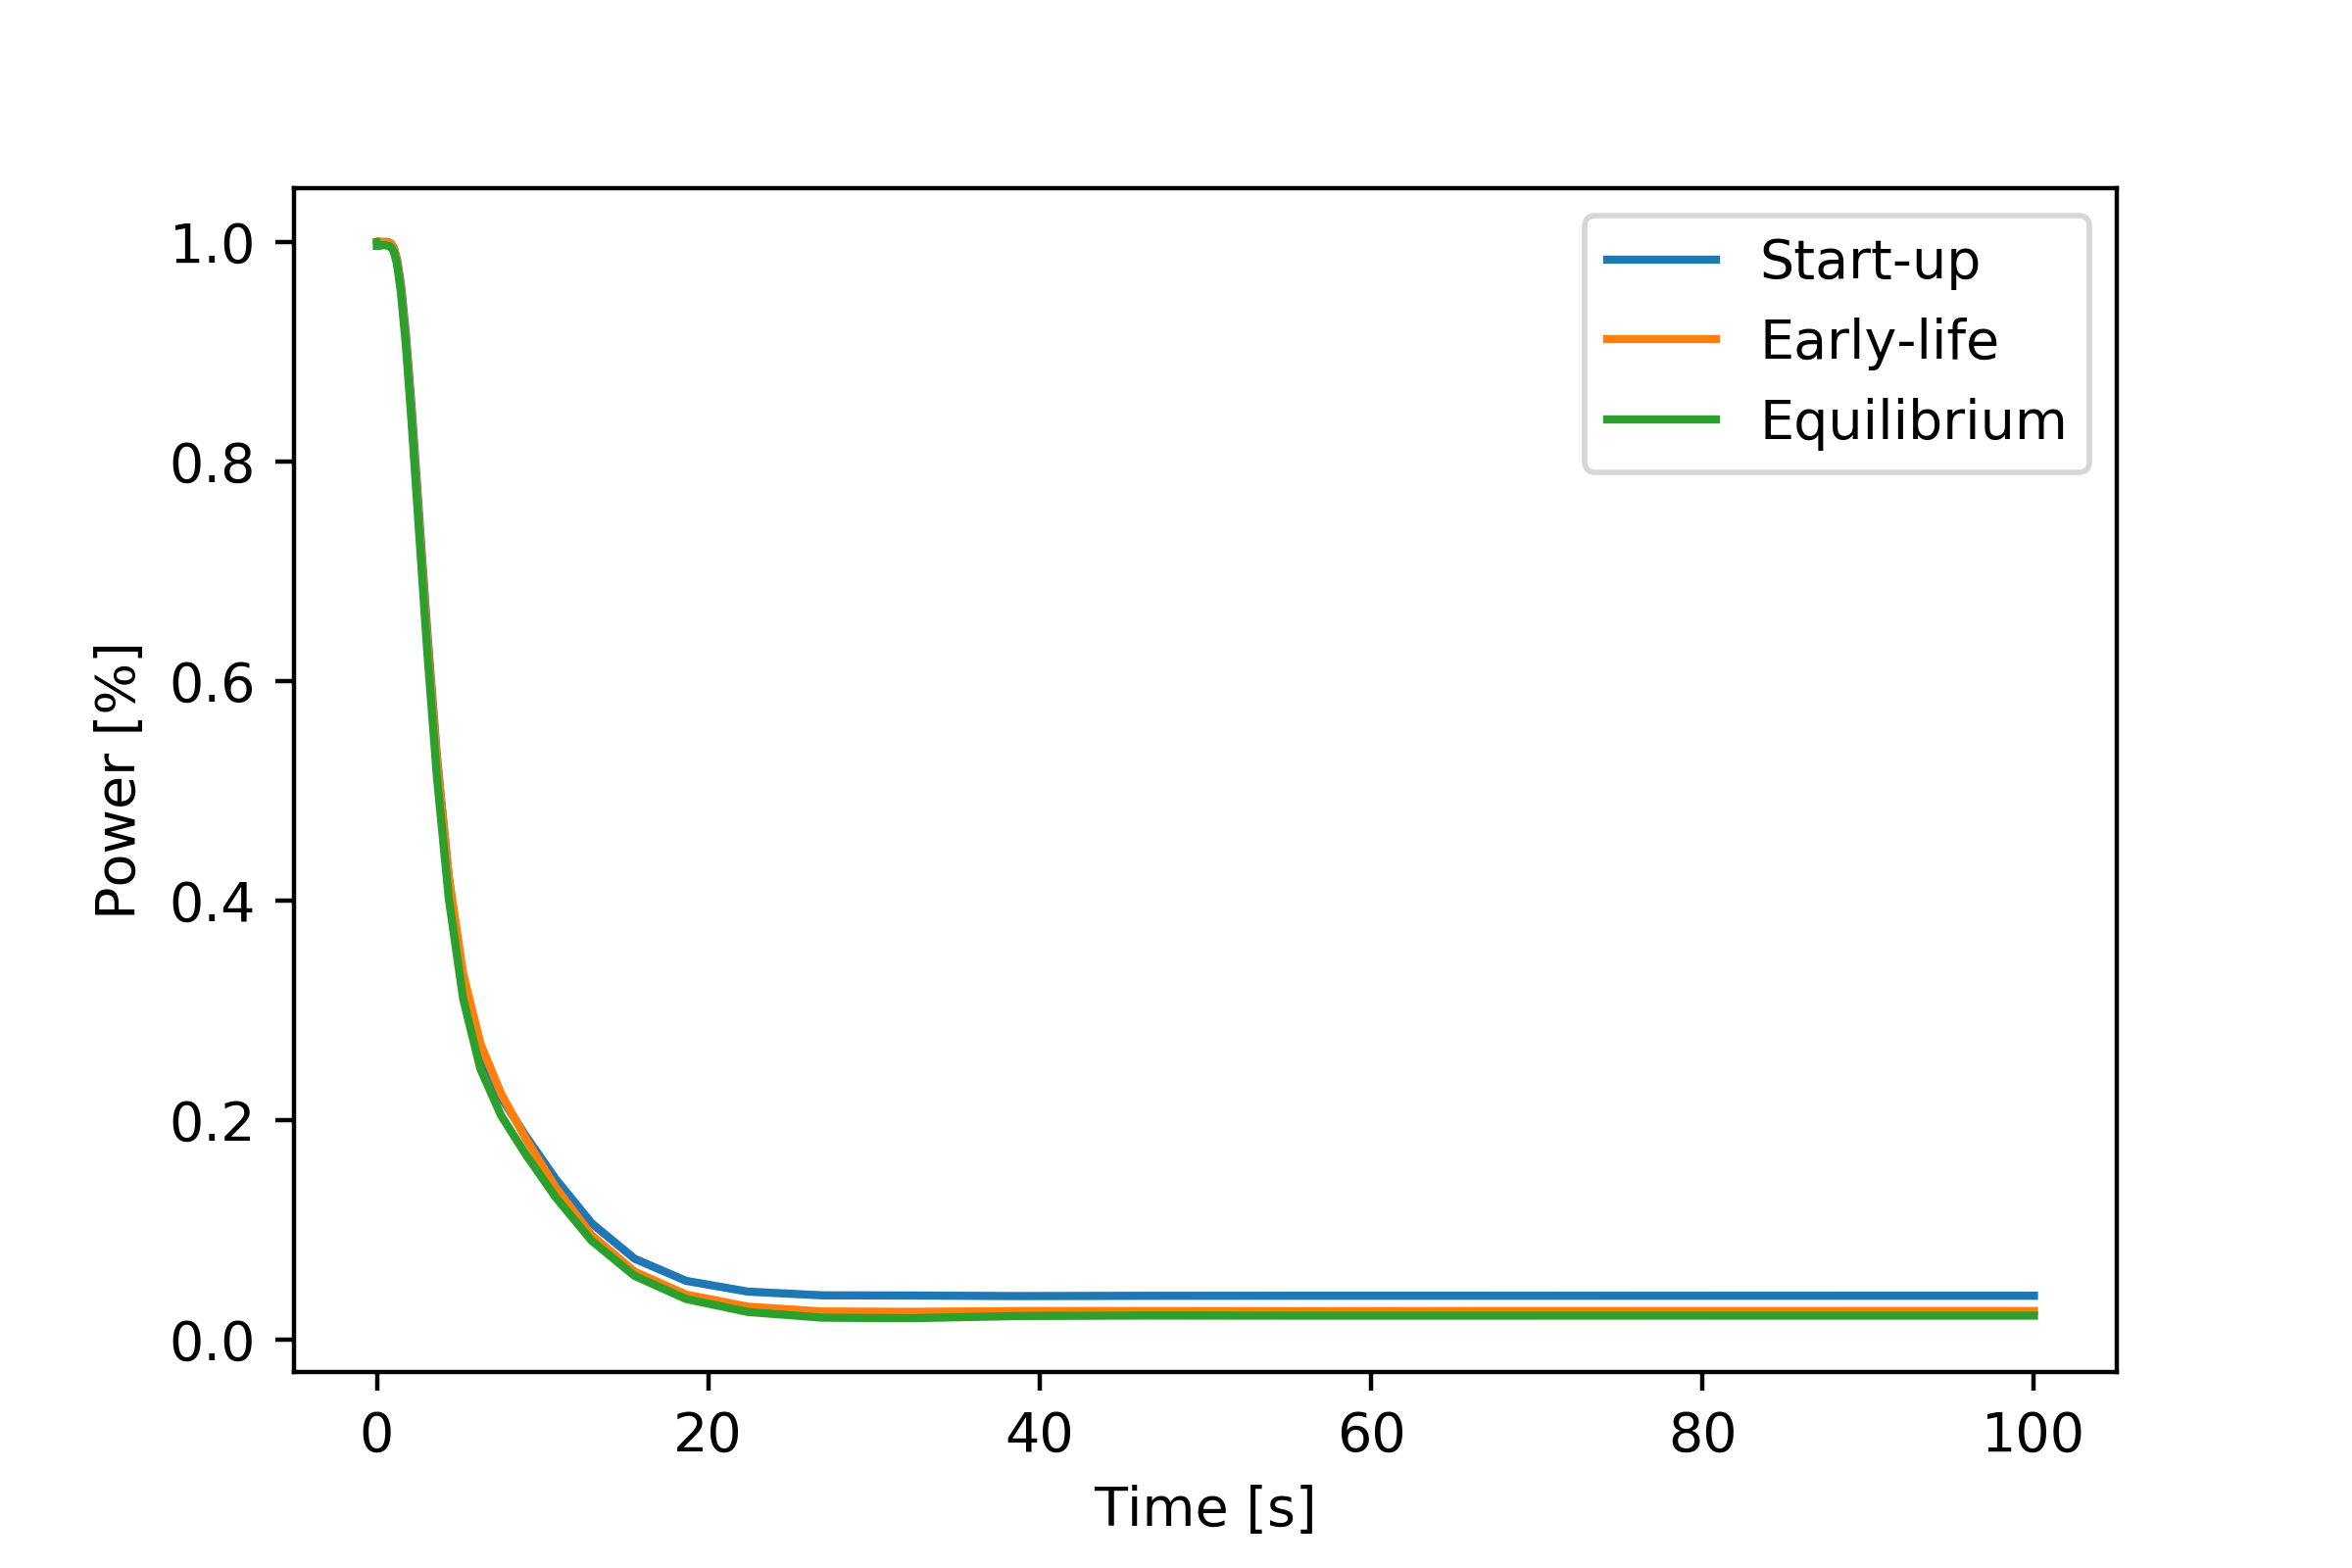
\includegraphics[width=.53\textwidth]{./figures/loscaheat}
	\captionsetup{justification=centering}
	\caption{Total thermal power generated, for start-up, \gls{BOL}, and
	 equilibrium fuel compositions during \gls{LOSCA}.}
	\label{fig:loscaheat}
\end{figure} 

	As observed in Figure \ref{fig:loscatemp}, the average fuel temperature
	increased by approximately 10 K and reached the new steady state
	30-40 s after \gls{LOSCA} began. While the time delay, due to the high
	initial
	\gls{DNP} concentration, is in good agreement with results reported by
	Fiorina et al. \cite{fiorina_modelling_2014}, the temperature rise is much
	smaller than the 100 K increase reported by the same authors.
	Power generation fell by two orders of
	magnitude, resulting in a negligible temperature difference between the
	inlets and outlets for all three fuel compositions. This could also be
	attributed to the relatively small total power of 2 GW discussed in the
	previous section, and the truncated \gls{MSFR} model.
	
	In comparing the three fuel compositions, a \gls{MSFR} loaded with
	start-up fuel composition is at a higher risk as it has higher
	temperatures under normal operating conditions and accident scenarios.

\section{Conclusion}

	Summarise results
	
	Safe
	
	Further development of the models is necessary to improve the accuracy
	and reliability of Moltres as a coupled neutronics/thermal-hydraulics code.
	Further work includes using an arbitrarily defined velocity profile, such
	as a parabolic profile. A better option would be to 

\bibliographystyle{ans}
\bibliography{bibliography}

\end{document}
